\documentclass[10pt,leter,openany]{article}
\usepackage[latin1]{inputenc}
\usepackage[english]{babel}
\usepackage{amsmath}
\usepackage{amsfonts}
\usepackage{amssymb}
\usepackage{graphicx}
\usepackage{listings}
\usepackage{color}
\usepackage[left=3cm,right=3cm,top=3cm,bottom=3cm]{geometry}
\usepackage[numbers,sort&compress]{natbib}
\usepackage{url}
\usepackage{caption}
\usepackage{siunitx}
\usepackage{subfigure}
\usepackage{float}
\usepackage{booktabs}

\usepackage{comment}

\setlength{\parindent}{0pt}
\setlength{\parskip}{4pt}

\definecolor{mygreen}{rgb}{0,0.6,0}
\definecolor{mygray}{rgb}{0.5,0.5,0.5}
\definecolor{mymauve}{rgb}{0.58,0,0.82}

\lstset{ 
	backgroundcolor=\color{white},   % choose the background color; you must add \usepackage{color} or \usepackage{xcolor}; should come as last argument
	basicstyle=\footnotesize,        % the size of the fonts that are used for the code
	breakatwhitespace=false,         % sets if automatic breaks should only happen at whitespace
	breaklines=true,                 % sets automatic line breaking
	captionpos=b,                    % sets the caption-position to bottom
	commentstyle=\color{mygreen},    % comment style
	deletekeywords={...},            % if you want to delete keywords from the given language
	escapeinside={\%*}{*)},          % if you want to add LaTeX within your code
	extendedchars=true,              % lets you use non-ASCII characters; for 8-bits encodings only, does not work with UTF-8
	firstnumber=01,                	 % start line enumeration with line 1000
	frame=single,	                 % adds a frame around the code
	keepspaces=true,                 % keeps spaces in text, useful for keeping indentation of code (possibly needs columns=flexible)
	keywordstyle=\color{blue},       % keyword style
	language=Python,                 % the language of the code
	morekeywords={*,...},            % if you want to add more keywords to the set
	numbers=left,                    % where to put the line-numbers; possible values are (none, left, right)
	numbersep=5pt,                   % how far the line-numbers are from the code
	numberstyle=\tiny\color{mygray}, % the style that is used for the line-numbers
	rulecolor=\color{black},         % if not set, the frame-color may be changed on line-breaks within not-black text (e.g. comments (green here))
	showspaces=false,                % show spaces everywhere adding particular underscores; it overrides 'showstringspaces'
	showstringspaces=false,          % underline spaces within strings only
	showtabs=false,                  % show tabs within strings adding particular underscores
	stepnumber=1,                    % the step between two line-numbers. If it's 1, each line will be numbered
	stringstyle=\color{mymauve},     % string literal style
	tabsize=2,	                     % sets default tabsize to 2 spaces
	title=\lstname                   % show the filename of files included with \lstinputlisting; also try caption instead of title
}


\usepackage[dvipsnames]{xcolor}

\usepackage{fancyvrb}

% redefine \VerbatimInput
\RecustomVerbatimCommand{\VerbatimInput}{VerbatimInput}%
{fontsize=\footnotesize,
	%
	frame=lines,  % top and bottom rule only
	framesep=2em, % separation between frame and text
	rulecolor=\color{Gray},
	%
	label=\fbox{\color{Black}data.txt},
	labelposition=topline,
	%
	commandchars=\|\(\), % escape character and argument delimiters for
	% commands within the verbatim
	commentchar=*        % comment character
}


\usepackage{titling}
\newcommand{\subtitle}[1]{%
	\posttitle{%
		\par\end{center}
	\begin{center}\large#1\end{center}
	\vskip0.5em}%
}


\author{5273}
\title{Homework Assignment 5: Applied Probabilistic Models}
\subtitle{Aspects of Normal Distribution and Pseudo-random Numbers }
\date{}



\begin{document}
	
\maketitle

\section{Introduction}
	
	In this work, it is studied the generation of pseudo-random numbers by different algorithms. Also, several experiments have been used to generate normal distributions from those generation methods. The algorithm's sensitivity is also tested changing parameters, and variables that define the different forms of generations are also part of the study.
	
	For the analysis, it is used the R software in its version 4.0.2 \citep{r}, and the code used is available on the GitHub repository \citep{github}. This work is run on a MacBook Air with an Intel Core i5 CPU $ @ $ 1.8 GHz and 8 GB RAM.
	
\section{Algorithms}
	 
	It is implemented the Box-Muller transform \citep{box1958note}, which from two numbers uniformly distributed, generates normally distributed ones. Those numbers should be independent, but some tests are performed with several dependencies to see this algorithm's behavior. For this procedure, the following code is used, which creates a function that returns a pair of values resulting from applying the corresponding equations. 
	
	\lstinputlisting[language=R, firstline=17, lastline=23]{codes/a5.R}
	
	As can be seen, it takes two uniformly distributed random numbers using the function \texttt{runif} from R as a source, and it generates a pair of independent, normally distributed pseudo-random numbers.
	
	On the other hand, it is analyzed the Linear Congruential Generator (LCG) \citep{l2017history}, which is an algorithm that generates a sequence of pseudo-randomized numbers. This method is computed using the following code. This algorithm is defined by the seed or initial value ($X_{0}) $, a modulus ($m$), a multiplier ($a$), and an increment ($c$) . 
	
	
	\lstinputlisting[language=R, firstline=25, lastline=36]{codes/a5.R}
	
\section{Experiments}
	
	Experiments for this work are based on the generation of Normal distributions from different methods. Several variations are studied to test the sensitivity of these algorithms as well. The parameters are the number of repetitions or sample size ($ n $) with a value of 1000, then a mean ($\mu$) of 10, a standard deviation ($\sigma$) of 2, and a seed of 27. Those values are arbitrarily selected at first and will be changed for further sensitivity analysis. 
	
	\subsection{Box-Muller Transform}
	
		The first experiment is performed with the Box-Muller transform. This method generates a sequence of uniformly distributed values. This generation of pseudo-random numbers uses the elements generated by the variable $Z_{0}$. The same procedure is executed with the variable $Z_{1}$, and both distributions are compared with the generated using the \texttt{rnorm} function of R. This comparison is shown in Figure \ref{fig:dens1}.
	
			\begin{figure}
				\begin{center}
					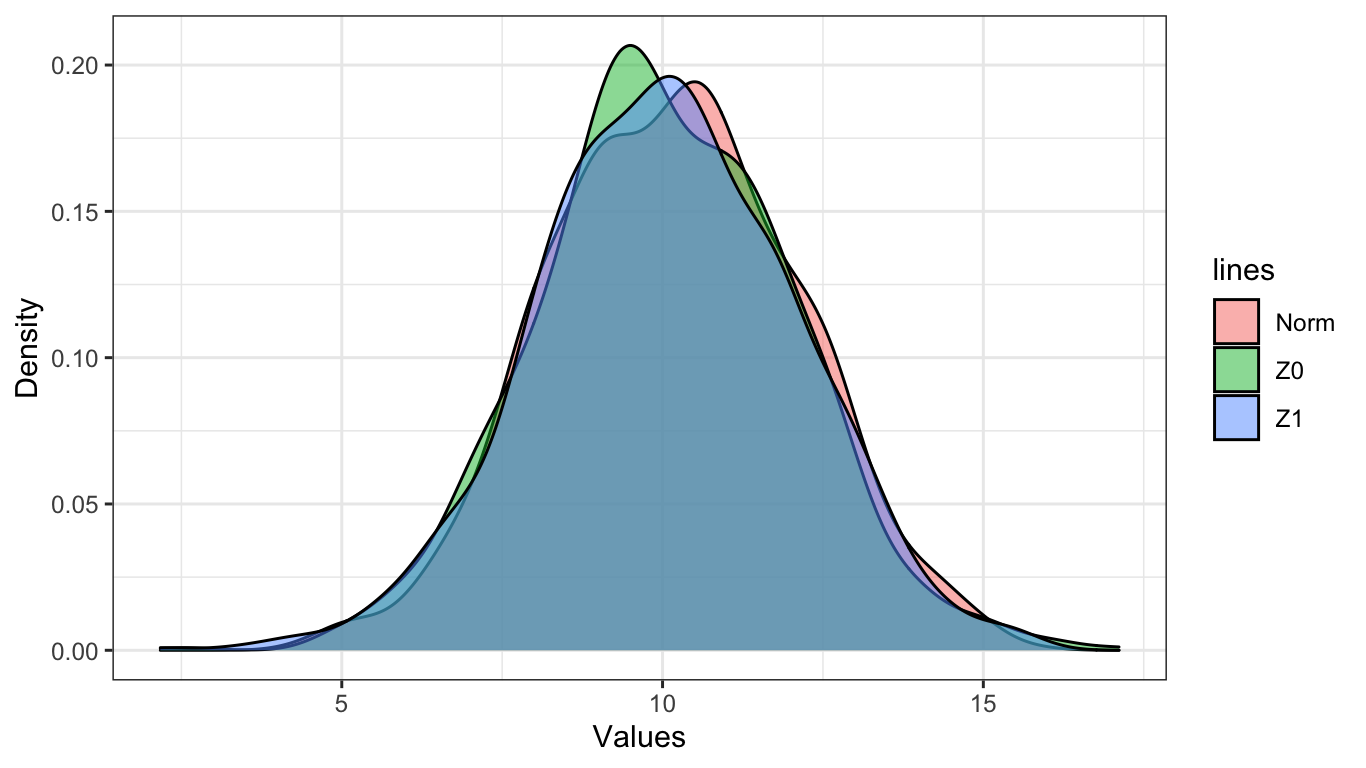
\includegraphics[scale=0.29]{extras/densplot1}
					\captionof{figure}{Density Plot of Normal Distributions}
					\label{fig:dens1}
				\end{center}
			\end{figure}
		
		
		To perform a sensibility analysis for this algorithm, the parameters $\mu$ and $\sigma$ were changed, and Shapiro Test is performed 30 times for each combination. An example of the results of one experiment is shown in Table \ref{tab:gaussian_mu_sigma}. As a result of the test, it is important to highlight that it passed in all repetitions for every test, except for Test 3, in which the algorithm had a $p$-value less than 0.05 in two times.
		
		
		\begin{table}[]
			\centering
			\caption{Result of one experiment of the Shapiro test changing values of $\mu$ and $\sigma$.}
			\label{tab:gaussian_mu_sigma}
			\begin{tabular}{lrrr}
				\hline
				& \multicolumn{1}{c}{$\mu$} & \multicolumn{1}{c}{$\sigma$} & \multicolumn{1}{c}{$p$-value} \\ \hline
				Test 1  & 400                       & 20                           & 0.548                         \\
				Test 2 & 225                       & 7                            & 0.3549                        \\
				Test 3 & 3                         & 0.25                         & 0.0860                        \\
				Test 4 & -23                       & 3                            & 0.5139                        \\
				Test 5 & -100                      & 12                           & 0.2405                        \\ \hline
			\end{tabular}
		\end{table}
	
	
		In addition, it is generated a boxplot of these distributions (see Figure \ref{fig:box1}), and an analysis of variance (ANOVA) of one way is performed. In the ANOVA test, the null hypothesis ($ H_{0} $)  implies that there is not enough evidence to prove the mean of the group is different from another. And the alternative hypothesis ($ H_{1} $) that at least, the mean of one group is different. In this case, the $p$-value is greater than 0.05, so there is no evidence to reject the null hypothesis, and therefore it is concluded that the means are identical.
 
			\begin{figure}
				\begin{center}
					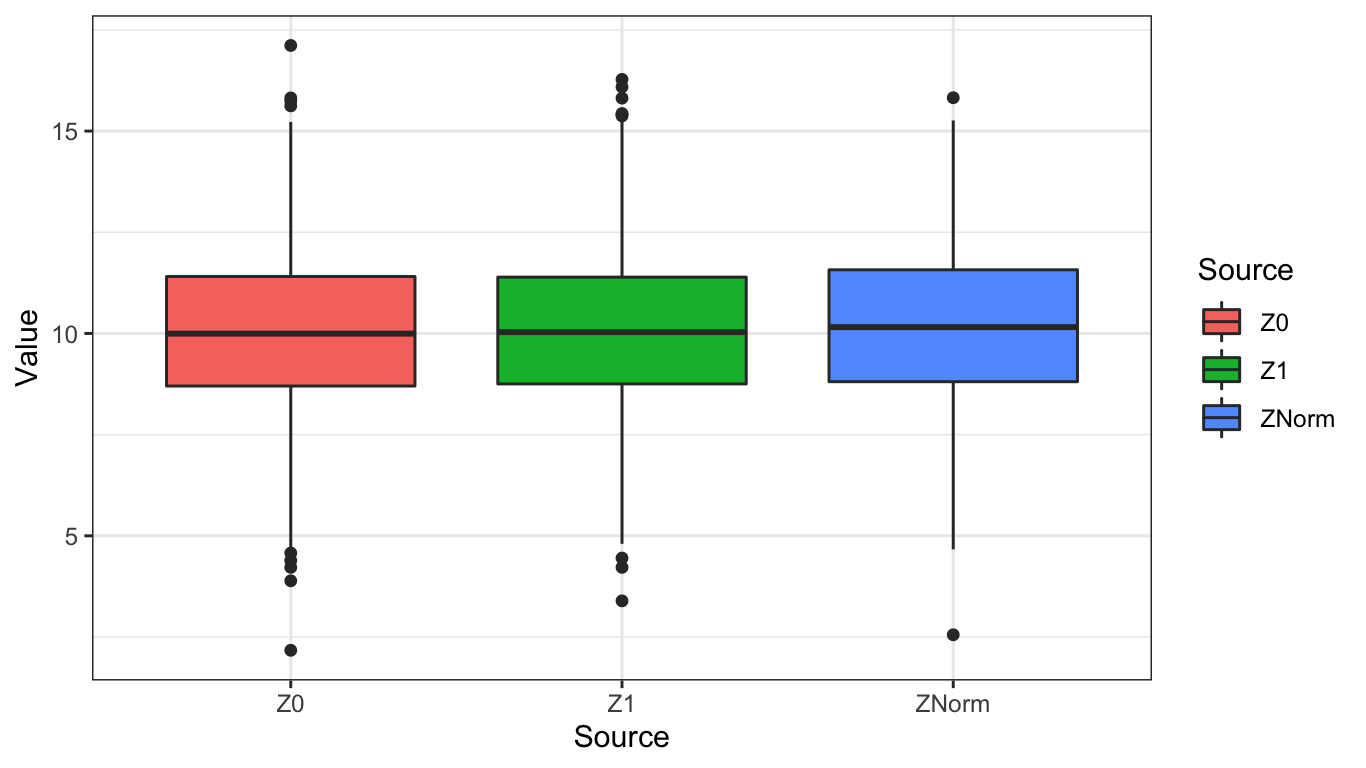
\includegraphics[scale=0.29]{extras/boxplot1}
					\captionof{figure}{Box Plot of Normal Distributions}
					\label{fig:box1}
				\end{center}
			\end{figure}

		\vspace{0.7cm}
		\VerbatimInput{extras/aov.txt}
		

	\subsubsection{Testing Independency of the uniform pseudo-random generated numbers}

		A sensitivity analysis changing different relations between the uniformed pseudo-random numbers $ u_{1} $ and $ u_{2} $ from the Box-Muller transform is performed. Changes in which the algorithm is subject are defined by how the uniform pseudo-random numbers are generated. Then the transform is performed and repeated 1000 times, and a Shapiro-Test is performed to test the normality of these different generations. These changes are detailed in Table \ref{tab:dep}. In those cases, the algorithm only kept generating normal distributions if the relation is the difference between $ u_{1}$ and $ u_{2} $, and when it is generated a number $ u_{2} $ between 1 and 10 (it can be considered as a bigger number), and it is subtracted with a multiple of $u_{1}$.


		\begin{table}[]
			\centering
			\caption{Results of Shapiro Test with different relations.}
			\label{tab:dep}
			\begin{tabular}{@{}lr@{}}
				\toprule
				Dependency                     & $ p $-value   \\ \midrule
				$ u_{2} $\textgreater{}$u_{1}$             & $ 2.67\times 10^{-13} $ \\
				$ u_{2} $ = $u_{1}$-\texttt{runif(1)}               & 0.3877    \\
				$ u_{2} $ = \texttt{runif(1,1,10)}-2$u_{1}$ & 0.6331    \\
				$ u_{2} $ = (\texttt{runif(1)}-$u_{1}$)/$u_{1}$          & 0.0186    \\
				$ u_{2} $ = 2$u_{1}$                     & $ 4.5\times10^{-16} $ \\
				$ u_{2} $= $u_{1}$*\texttt{runif(1)}               & $2.35 \times 10^{-13}$ \\ \bottomrule
			\end{tabular}
		\end{table}

	\subsection{Linear Congruential Generator}

		Experiments with the LCG are performed based on the uniformed pseudo-random sequence generate with this algorithm. It is tested the distribution of the data with the Chi-squared test provided by the \texttt{uniform.test()} function over the histogram of the data. For this test, the $p$-value is greater than 0.05, so there is no evidence to reject the null hypothesis, and the data might be uniformly distributed.

   		\VerbatimInput{extras/unif_test.txt}

	\subsubsection{Using LCG in the  Box-Muller Transform}

		After concluding that data generated are uniformly distributed, it could be used to test these values in the Box-Muller transform as the values $ u_{1} $ and $u_{2}$. 
		The results of the histogram of this experiment are shown in Figure \ref{fig:hist2}. It can be seen with a higher probability the normality of the data using the Box-Muller transform with those values. Shapiro Test throws a $p$-value of  0.4087, so it can be concluded data may proceed from a normal distribution.


		\begin{figure}
			\begin{center}
				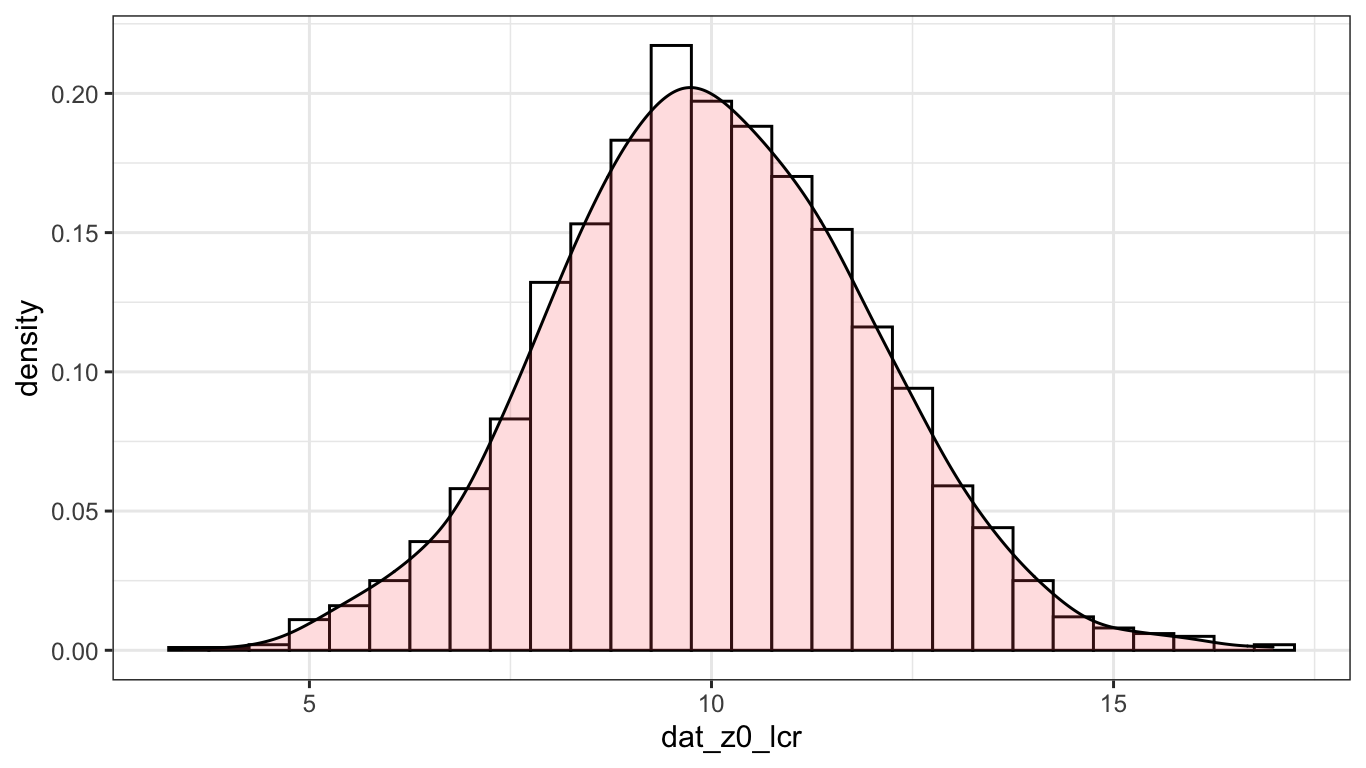
\includegraphics[scale=0.30]{extras/hist2}
				\captionof{figure}{Histogram of the Box-Muller Transform using the LCG}
				\label{fig:hist2}
			\end{center}
		\end{figure}


		Other experiments are performed, for example, changing the values of $ a $, $ c $, and $ m $, resulting in the loss of normality when those values decrease with the same seed. This tests are shown in Table \ref{tab:muller_acm}.


			\begin{table}[]
				\centering
				\caption{Results of the Shapiro Test changing the values $a$, $c$, and $m$.}
				\label{tab:muller_acm}
				\begin{tabular}{@{}lrrrr@{}}
					\toprule
					& \multicolumn{1}{l}{$ a $} & \multicolumn{1}{l}{$ c $} & \multicolumn{1}{l}{$ m $} & \multicolumn{1}{l}{$ p $-value} \\ \midrule
					Test 1  & 3067                  & 4751                  & 7919                  & 0.2793                      \\
					Test 2 & 1993                  & 2293                  & 3001                  & 0.2514                      \\
					Test 3 & 1049                  & 1459                  & 1931                  & 0.9003                      \\
					Test 4 & 463                   & 701                   & 1033                  & 0.0091                      \\
					Test 5 & 229                   & 347                   & 461                   & $ 2.2\times 10^{-16} $                     \\ \bottomrule
				\end{tabular}
			\end{table}

		Table \ref{tab:muller_nonprime} also show experiments of different values of a, c, and m, but this time making them as non-prime values. Results show that with these numbers, it is susceptible to applying them into the gaussian algorithm because $p$-values show in multiple tests that the generated sequence is not normally distributed. 


			\begin{table}[]
				\centering
				\caption{Results of the Shapiro test with non prime values of $a$, $ c$, and $m$.}
				\label{tab:muller_nonprime}
				\begin{tabular}{@{}lrrrr@{}}
					\toprule
					& \multicolumn{1}{c}{$ a $} & \multicolumn{1}{c}{$ c $} & \multicolumn{1}{c}{$ m $} & \multicolumn{1}{l}{$ p $-value} \\ \midrule
					Test 1  & 11000                 & 27070                 & 39720                 & 0.06912                     \\
					Test 2 & 11343                 & 20505                 & 35100                 & $ 2.2 \times 10^{-16}   $                   \\
					Test 3 & 15250                 & 35400                 & 65104                 & $ 4.97\times 10^{-5} $                   \\
					Test 4 & 5640                  & 10240                 & 15800                 & $ 1.83 \times 10^{-9}  $                  \\
					Test 5 & 2505                  & 5005                  & 15145                 & $ 4.13\times 10^{-16}    $                 \\ \bottomrule
				\end{tabular}
			\end{table}

	\subsection{A nonlinear Generator}

		 Non-linear generators can be defined for example by using a nonlinear transition function $ f $, or a nonlinear output function $g$, or by combining two or more linear random linear generation, etc. In \citet{knuth2014art} it is analyzed a generator based on a quadratic recurrence of the form:
		 \begin{equation*}
		 	x_{i} = (ax_{i-1}^{2} + bx_{i-1} + c) \hspace{0.1cm}\text{mod} \hspace{0.1cm}  m
		 \end{equation*}
	 
		  
		  For this generator the author gave conditions for a maximal period of $m$. If  $m=2^{e}$, then the period is maximal if and only if $a$ is even, ($b-a-1$) mod $4 = 0$, and $c$ is odd. The code used for this method is shown below and  is adapted  to return values in the interval (0,1). It is also tested with the \texttt{uniform.test} function or R, with $p-value$ of 0.1459, evidencing uniformity in data.
 
		\lstinputlisting[language=R, firstline=11, lastline=23]{codes/knuth.R}
		
		\VerbatimInput{extras/knuth.txt}
	
	

 \clearpage

	\bibliography{assignment5}
	\bibliographystyle{plainnat}
	
\end{document}